\section{Entorno Operativo}

\subsection{Interoperabilidad de los sistemas }

La interoperabilidad es la capacidad de los sistemas y de los procedimientos a los que éstos dan soporte, de compartir datos y posibilitar el intercambio de información y conocimiento entre ellos. 

La interoperabilidad entre los sistemas y organizaciones civiles y militares, aumenta la capacidad en el espacio aéreo congestionado, mejora los niveles de seguridad, aumenta la eficiencia de los vuelos y contribuye a la provisión ATS óptima a compartir una base técnica y operacional común. Esta interoperabilidad proporciona beneficios para la aviación civil y militar y posibilita la introducción de sistemas más avanzados.

Para que la interoperabilidad de los sistemas se lleve a cabo es necesario que los procesos de certificación sean comunes entre ambas partes (civil y militar). Por ello, será necesario implementar un nuevo proceso de certificación alternativo que permita utilizar las capacidades militares disponibles para cumplir con los requisitos civiles CNS / ATM civiles. Cuando no sea posible alcanzar la interoperabilidad entre sistemas será necesario definir procedimientos específicos capaces de solucionar estos problemas. Por ejemplo, el aumento de la separación entre aeronaves civiles y militares, en caso de que las aeronaves militares no pudieran cumplir con determinadas prestaciones de navegación.

En cuanto a los sistemas que van a requerir un funcionamiento conjunto son: 

\begin{itemize}
    \item Los sistemas de comunicación.
    \item Los sistemas de navegación.
    \item Los sistemas de vigilancia.
\end{itemize}

\subsubsection{Sistemas de comunicación}

La homogeneización en los sistemas de comunicación será un punto calve para la coordinación civil-militar y permitirá el intercambio de datos e información de una forma segura para que la operaciones se lleven a cabo de una forma eficiente.

\begin{enumerate}
    \item \textbf{Comunicaciones tierra-tierra:}
    
    En la actualidad, la mayoría de las unidades militares dependen de la \acrfull{aftn} de la OACI o de la \acrfull{cidin} para recibir información aeronáutica, NOTAM, datos meteorológicos, etc. 
    
    La AFTN utiliza dos tipos de estaciones fijas aeronáuticas: centros de comunicaciones AFTN y estaciones AFTN. El centro de comunicaciones AFTN es una estación AFTN cuya función principal es retransmitir mensajes AFTN hacia o desde varias otras estaciones AFTN interconectadas.

    En la mayoría de los aeródromos donde se proporciona ATS, hay una estación AFTN. Varias de estas estaciones agrupadas y alrededor de un centro AFTN forman un circuito AFTN.
    
    \begin{figure}[H]
        \centering
        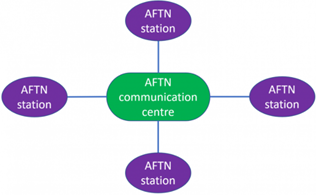
\includegraphics[width=0.5\linewidth]{figuras/aftn.png}
        \caption{Organización de un sistema AFTN.}
        \label{fig:aftn}
    \end{figure}
    
    A medida que aumenta la demanda de capacidad y aumentan las presiones económicas y ambientales, es más importante que nunca que los proveedores de servicios de navegación aérea (ANSP) compartan información precisa y oportuna. Durante muchos años, la Red de telecomunicaciones fijas aeronáuticas (AFTN) ha desempeñado un papel fundamental al permitir que los ANSP intercambien mensajes que faciliten los viajes aéreos seguros. Sin embargo, la tecnología obsoleta y las capacidades de comunicación limitadas de AFTN hacen que sea cada vez más difícil satisfacer las necesidades de un dominio en crecimiento al compartir de manera efectiva información aeronáutica y meteorológica, incluidos planes de vuelo, avisos a los aviadores (NOTAM) y boletines meteorológicos.

    Por tanto, será necesario dar paso a las estructuras del sistema (AMHS) que convertirán en un requisito de interoperabilidad civil-militar tan pronto como AFTN sea reemplazado gradualmente por AMHS.
    
    Por último, se están introduciendo redes basadas en el Protocolo de Internet (IP) y el acceso a su infraestructura se convertirá en un requisito de interoperabilidad civil-militar. Esto permitirá servicios más avanzados, incluida la gestión de información en todo el sistema (SWIM). Sin embargo, el uso militar del componente SWIM de esta infraestructura dependerá, entre otras cosas, de las disposiciones de seguridad adecuadas.
    
    La evolución de los sistemas de comunicación tierra-tierra deberán seguir la evolución mostrada en la figura (\ref{fig:evolucion}) y, además, tanto aeronaves civiles como militares harán uso de esta tecnología a medida que se vayan implementando.
    
    \begin{figure}[H]
        \centering
        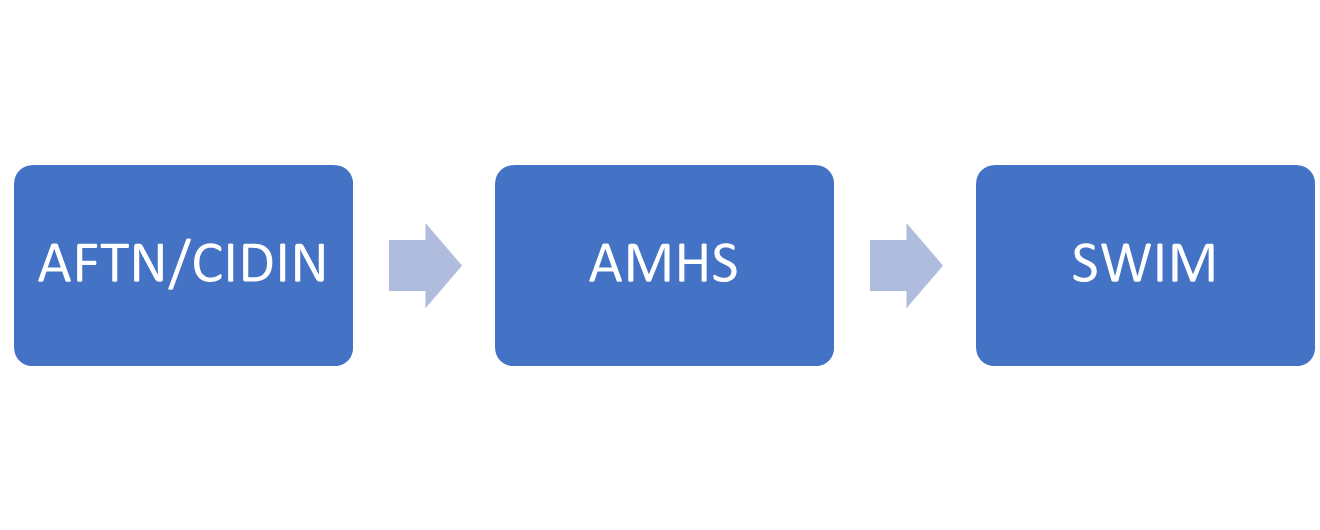
\includegraphics[width=0.5\linewidth]{figuras/evolucion.png}
        \caption{Evolución de los sistemas tierra-tierra.}
        \label{fig:evolucion}
    \end{figure}

    \item \textbf{Comunicaciones aire-tierra:}
    
    Para las comunicaciones de datos aire-tierra, la adquisición de capacidades de enlace de datos para \acrfull{cpdlc} debería facilitar un uso más eficiente del espacio aéreo que requiere dicha capacidad. Sin embargo, se espera que muchas aeronaves estatales soliciten exenciones de los requisitos de equipamiento de enlace de datos, debido a los requisitos de la misión y los desafíos del ajuste hacia adelante.

    Además, para asegurar la coordinación operativa, especialmente en situaciones de emergencia, los ATS civiles, las unidades militares apropiadas y sus unidades de defensa aérea deben estar conectados por circuitos de voz directos o su equivalente digital. Para mejorar la seguridad y la eficiencia, la voz debe complementarse con una notificación electrónica entre centros, coordinación y transferencia de mensajes de acuerdo con las normas vigentes para la aviación civil.

\end{enumerate}

\subsubsection{Sistemas de navegación}

Los sistemas de Navegación constituyen otro pilar importante, donde la interoperabilidad entre los sistemas utilizados por la parte militar y civil resulta imprescindible para la implantación de AFUA. Los sistemas que deberán tener una base común para todos los participantes del espacio aéreo son los siguientes:

\begin{enumerate}
    \item \textbf{Perfomance Based Navigation (PBN):}
    
    El \acrfull{pbn} es un nuevo concepto basado en el uso de los sistemas de navegación de área (RNAV). 

    La navegación basada en el desempeño según OACI, hace necesario que los sistemas de desempeño requeridos en navegación (RNP) y navegación de área (RNAV) sean definidos según los términos de precisión, integridad, disposición, continuidad y funcionalidad requeridos para las operaciones propuesta en el contexto de un espacio aéreo particular, cuando está respaldado por una infraestructura de navegación apropiada (GNSS u otro tipo de infraestructura aplicable a la navegación).
    
    El concepto PBN, incluyendo el uso de señales obtenidas de satélites para las actuaciones en ruta y aproximación, está reemplazando gradualmente al sistema tradicional de navegación apoyada en ayudas terrestres a la navegación.
    
    El concepto de PBN está compuesto de tres partes:
    
    \begin{enumerate}
        \item Las especificaciones de navegación. Describen los requisitos de desempeño en términos de precisión, integridad y continuidad de las operaciones propuestas en un determinado espacio aéreo. También describe cómo se van a alcanzar estos requisitos. Deben llevar asociado unos apropiados estándares de conocimiento por parte de los pilotos, así como formación adecuada.
        
        \item La infraestructura de ayudas a la navegación que se utilizarán para cumplir con las especificaciones de navegación. La disponibilidad de esta infraestructura de ayuda tiene que ser tenida en cuenta a la hora de habilitar la aplicabilidad de este tipo de navegación.
        
        \item La aplicación a la navegación está referida a las especificación y ayudas a la navegación en el contexto de un espacio aéreo con rutas ATS y procedimientos de vuelo por instrumentos.
    \end{enumerate}
    
    Los beneficios asociados a la implantación del concepto PBN son los siguientes:
    
    \begin{itemize}
        \item Reduce la necesidad de mantener una serie de ayudas específicas para la navegación y ruta y los costes asociados del uso y mantenimiento de estas.
        \item Evita la necesidad de desarrollar ayudas específicas para las operaciones con cada nueva evolución de los sistemas de navegación, lo que supone un coste demasiado elevado.
        \item Permite usar el espacio aéreo con una mayor eficiencia.
    \end{itemize}
    
    \item \textbf{Global Navigation Satellite System (GNSS):}
    
    El \acrfull{gnss} transmite rangos de señales que se utilizan para el posicionamiento y localización de cualquier parte del globo terrestre. Estos satélites permiten determinar coordenadas geográficas y altitud en un punto dado.

    El origen de este sistema es militar. La navegación por satélite permitía alcanzar valores de precisión que no se habían conseguido obtener con anterioridad, esto permitía aumentar la precisión sobre objetivos militar, aumentando la efectividad y reduciendo daños no deseados.
    
    En el ámbito civil, los sistemas de posicionamiento por satélite son reconocidos como un elemento clave en los sistemas de comunicación, navegación y vigilancia (CNS). 
    
    El GNSS comprende a todos los sistemas de navegación por satélite, los que ya han sido implementados (GPS y GLONASS) y los que están en desarrollo (GALILEO). Permiten la utilización de las redes de satélite como soporte a la navegación, ofreciendo una localización precisa de las aeronaves.
    
    Cuando se encuentre plenamente desarrollado se prevé que pueda ser utilizado, en todas las fases de la operación de una aeronave, sin requerir ayuda de cualquier otro sistema de navegación convencional.
    
    \item \textbf{Instrumental Landing System (ILS) y Microwave Landing System (MLS):}
    
    El \acrfull{ils} es el sistema de ayuda a la aproximación y aterrizaje establecido por OACI. Este sistema permite que un avión sea guiado con presión durante la aproximación a la pista, y en algunos casos, a lo largo de la misma.

    El ILS está formado por dos subsistemas independientes, uno permite proporcionar guiado lateral, y el otro proporciona guía vertical. Se trata del localizador y la senda de planeo respectivamente.
    
    El tipo de operaciones que permite el uso del ILS son las siguientes:
    
    \begin{itemize}
        \item \textbf{Categoría I:} Altura de decisión no inferior a 60 m (200 ft) y con una visibilidad de no menos de 800 m o con un alcance visual en la pista no inferior a 550 m.
        \item \textbf{Categoría II:} Altura de decisión inferior a 60 m (200 ft) pero no inferior a 30 m (100 ft) y con un alcance visual en la pista no inferior a 300 m.
        \item \textbf{Categoría III:}
        \begin{itemize}
            \item \textbf{Categoría IIIA:} Altura de decisión inferior a 30 m (100 ft), o sin altura de decisión y un alcance visual en la pista no inferior a 175 m.
            \item \textbf{Categoría IIIB:} Altura de decisión inferior a 15 m (50 ft), o sin altura de decisión, y un alcance visual en la pista inferior a 175 m pero no inferior a 50 m.
            \item \textbf{Categoría IIIC:} Sin altura de decisión y sin restricciones de alcance visual en la pista.
        \end{itemize}
    \end{itemize}
    
    Por su parte, el MLS, es un sistema de ayuda al aterrizaje desarrollado por el servicio militar de EEUU, cuya principal misión es paliar una de las mayores limitaciones del sistema ILS. Trata de solucionar los problemas ocasionados por la presencia de irregularidades en el terreno y las distorsiones ocasionales.
    
    Algunas de las ventajas proporcionadas por el MLS son las siguientes:
    
    \begin{itemize}
        \item Equipamiento más preciso.
        \item Permite múltiples curvas de aproximación, a diferencia de la rigidez de la aproximación lineal del ILS.
        \item Es más barato.
    \end{itemize}
    
    Ambos sistemas serán sustituidos en el futuro por sistemas de navegación por satélite basados en GNSS, que son mucho más precisos que ambos.
\end{enumerate}

\subsubsection{Sistemas de vigilancia}

En este parte, se describirá la interoperabilidad de los sistemas de vigilancia y la problemática que se deriva del uso de los diferentes sistemas.

Hay diferentes sistemas de vigilancia:

\begin{enumerate}
    \item \textbf{Vigilancia no cooperativa:}
    \begin{enumerate}
        \item \textbf{\acrfull{psr}:} Este sistema es un sistema de vigilancia independiente no cooperativa, es decir no es vulnerable a ataques informáticos ya que no comparte datos. 
        
        Las unidades de defensa aérea dependen de una amplia cobertura de radar de vigilancia primaria para detectar objetivos. 
        
        Las ventajas de utilizar el Radar primario son los siguientes:
        
        \begin{itemize}
            \item Aumenta la conciencia de la situación.
            \item La seguridad de todas las partes interesadas al agregar una capa de vigilancia.
            \item La capacidad para determinar el movimiento de aeronaves civiles cuando los transpondedores del radar secundario de vigilancia (SSR) no funcionan.
        \end{itemize}
    \end{enumerate}
    
    \item \textbf{Vigilancia cooperativa:} En esta sección se engloban los sistemas que son vulnerables a ataques electrónicos maliciosos e ilegales interferencia.
    \begin{enumerate}
        \item \textbf{\acrfull{ssr}:} SSR Mode S es el último radar de vigilancia secundario utilizado a nivel mundial. 
        
        Este sistema permite:
        
        \begin{itemize}
            \item El direccionamiento selectivo de aeronaves mediante el uso de una dirección de aeronave (24 bits) que identifica de forma única a cada aeronave.
            \item Tiene un enlace de datos bidireccional entre la estación terrestre y la aeronave, para el intercambio de información.
        \end{itemize}


        \item \textbf{\acrfull{adsb}:} es ante todo un medio de vigilancia, es decir, un medio para que el control del tráfico aéreo conozca la posición de los aviones. Nació de la observación de que los aviones modernos, gracias a los sistemas de posicionamiento por satélite (como GPS, GLONASS y pronto Galileo), conocen su posición con mucha más precisión que el control en tierra, porque los radares terrestres tienen una precisión limitada. Por tanto, la idea es que el avión calcule su propia posición y la envíe regularmente por radio.
        
        ADS-B funciona en modo broadcast. La aeronave envía regularmente su posición y otra información por radiodifusión a todos los usuarios interesados, normalmente al control en tierra, pero también a otras aeronaves si están equipadas con un receptor. La tasa de emisión de la posición depende de la fase de vuelo, por ejemplo, cada diez segundos en ruta y cada segundo en aproximación.
        
        El ADS-B es, por tanto, más que un medio de vigilancia, ya que permite a una aeronave equipada con ADS-B conocer la posición de otros aviones que la rodean, al menos aquellos que también están equipados con ADS-B. B. Además, los mensajes ADS-B no solo contienen la posición (3D), sino también otra información como identificación, velocidad, rumbo e intenciones.
        
        Una de las ventajas de ADS-B es que, dado que los aviones transmiten regularmente su posición de forma omnidireccional, ya no hay necesidad de radar: una antena de radio en tierra puede recibir estos mensajes (estación en modo S), mucho menos costosa que un radar. Por esta razón, el despliegue de ADS-B es una alternativa muy interesante en regiones no equipadas con radar.

        
        \begin{figure}[H]
            \centering
            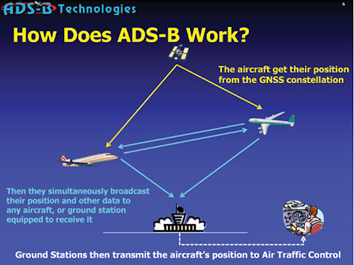
\includegraphics[width=0.5\linewidth]{figuras/adsb.png}
            \caption{Funcionamiento del ADS-B.}
            \label{fig:adsb}
        \end{figure}
        
        Una tecnica que combina las capacidades del sistema SSR Mode S con las de ADS-B es el de 1090 MHz extended squitter (1090 ES). Esto se logra utilizando un ES como enlace de transmisión de datos para transferir el informe ADS derivado de la aeronave.
        
        En cuanto a la interoperabilidad, hay que tener en cuenta que se espera que los militares equipen sistemas de seguridad (como \acrfull{acas}, \acrfull{gpws} y \acrfull{taws}) para aumentar la seguridad, reducir la infraestructura terrestre, el costo y la radio, y que permite entonces la interoperabilidad entre ellos.
        
        En cambio los beneficios serían los siguientes:
        
        \begin{itemize}
            \item La implementación coordinada de la infraestructura de vigilancia reduciría el costo total de vigilancia.
            \item Mayor redundancia con múltiples sistemas.
            \item Reducción de la necesidad de códigos especiales de interrogador de defensa aérea si se dispone de datos de identificación de vuelo civil a los militares.
            \item La disminución de la infraestructura cooperativa reduciría la carga de RF en las bandas de 1030/1090 MHz mejorar la calidad de los datos en aéreas de tráfico denso.
        \end{itemize}
        
        Los sistemas de vigilancia civil y militar comparten el mismo espectro de frecuencias. Para evitar la carga innecesaria de radiofrecuencia (RF) y la interferencia entre los sistemas de vigilancia utilizados para aplicaciones similares, la utilización de la frecuencia utilizada por dichos sistemas debe ser coordinada por las autoridades civiles y militares. Especialmente dado que las frecuencias 1 030 y 1 090 MHz admiten varios sistemas de vigilancia como SSR, ADS-B y ACAS, se reconoce la necesidad de limitar la carga de RF en las bandas 1 030/1 090 MHz. 
        
        También sería posible una reducción de la carga de radiofrecuencia mediante la cooperación estratégica entre las autoridades civiles y militares para garantizar la racionalización de la infraestructura de vigilancia general y mediante la coordinación de la utilización de frecuencias y la reducción de la extracción de datos a bordo con interrogatorios activos.
    \end{enumerate}
\end{enumerate}


\subsection{Entorno geopolítico}

La propia existencia del nacimiento del concepto \acrfull{fua} y su evolución en el concepto \acrfull{afua} es debido al contexto geopolítico en el que nace, Europa. En la otra zona del mundo que más se ha desarrollado la aviación, EEUU, este concepto no es tan necesario ya que todo el espacio aéreo pertenece al mismo país, el cual tiene un tamaño enorme. 

En cambio en Europa se tiene un espacio aéreo muy congestionado el cual está dividido por muchos estados. Los estados de la Unión Europea tienen un tamaño menos respecto a los presentes en otras zonas del mundo. En poco territorio se concentran muchos estados y cada uno tiene su ejercito y su soberanía respecto a su cielo. Esto hace que surjan los problemas derivados de las fronteras entre cada estado y que un vuelo pase por varios países cada uno con sus áreas restringidas para uso militar.

Es lógico que el concepto FUA haya surgido y tenido un mayor desarrolla en Europa, ya que es una zona con una problemática característica que el AFUA intenta solucionar.

\subsection{Instituciones}

El concepto del AFUA no es una idea abstracta que está en el aire sino que es un concepto creado, desarrollado y sustentado por un contexto social y unas instituciones en concreto. En este apartado se van a mencionar las más importantes respecto al AFUA con una pequeña descripción de ellas.

\subsubsection{SESAR Joint Undertaking}

El \acrfull{afua} se enmarca dentro del \acrfull{sesar}, que es un proyecto colaborativo para reformar completamente el espacio aéreo europeo y su gestión del tráfico aéreo (ATM). El programa actual lo gestiona la empresa SESAR Joint Undertaking como asociación público-privada.

El proyecto SESAR lo gestiona SESAR Joint Undertaking, una empresa creada en 2007 y  responsable de la coordinación y concentración de todas las actividades de investigación y desarrollo de la Unión Europea (UE) en materia de gestión del tráfico aéreo (ATM). Iniciado en 2004, el programa SESAR es el brazo tecnológico de la iniciativa del Cielo Único Europeo de la UE para integrar los sistemas de ATM de los Estados miembros.

La empresa común SESAR se creó con Eurocontrol y la Comisión Europea como miembros fundadores. Además de los dos miembros fundadores, 15 organizaciones han firmado un acuerdo de adhesión a la empresa común SESAR. El proyecto se enmarca dentro de la Red Transeuropea de Transporte.

\subsubsection{Comisión Europea}

La Comisión Europea (CE) es la rama ejecutiva de la Unión Europea, responsable de proponer legislación, hacer cumplir las leyes de la UE y dirigir las operaciones administrativas de la unión. Los comisarios prestan juramento en el Tribunal de Justicia Europeo en la ciudad de Luxemburgo, comprometiéndose a respetar los tratados y a ser completamente independientes en el desempeño de sus funciones durante su mandato.

\subsubsection{Eurocontrol}

La Organización Europea para la Seguridad de la Navegación Aérea, comúnmente conocida como Eurocontrol, es una organización internacional que trabaja para lograr una gestión del tráfico aéreo segura y sin fisuras en toda Europa. Fundada en 1960, Eurocontrol cuenta actualmente con 41 Estados miembros y tiene su sede en Bruselas (Bélgica). También cuenta con varias sedes locales, como las actividades de I+D en Brétigny-sur-Orge (Francia), el Instituto de Formación en Navegación Aérea (IANS) en Luxemburgo y el Centro de Control de la Zona Superior de Maastricht (MUAC) en Maastricht (Países Bajos). 

Aunque Eurocontrol no es una agencia de la Unión Europea, la UE ha delegado parte de su normativa sobre el Cielo Único Europeo en Eurocontrol, lo que la convierte en la organización central de coordinación y planificación del control del tráfico aéreo para toda Europa. La propia UE es signataria de Eurocontrol y todos los Estados miembros de la UE son actualmente también miembros de Eurocontrol. La organización trabaja con las autoridades nacionales, los proveedores de servicios de navegación aérea, los usuarios del espacio aéreo civil y militar, los aeropuertos y otras organizaciones. Sus actividades abarcan todas las operaciones de los servicios de navegación aérea de puerta a puerta: gestión estratégica y táctica del flujo, formación de controladores, control regional del espacio aéreo, tecnologías y procedimientos a prueba de seguridad y recaudación de las tasas de navegación aérea.

\subsubsection{Red Transeuropea de Transporte}

La Red Transeuropea de Transporte es una red prevista de carreteras, ferrocarriles y aeropuertos en la Unión Europea. La red forma parte de un sistema más amplio de redes transeuropeas, que incluye una red de telecomunicaciones y una red energética propuesta. La Comisión Europea adoptó los primeros planes de acción sobre redes transeuropeas en 1990.

La red prevé la mejora coordinada de carreteras primarias, ferrocarriles, vías navegables interiores, aeropuertos, puertos marítimos, puertos interiores y sistemas de gestión del tráfico, proporcionando rutas integradas e intermodales de larga distancia y alta velocidad. La decisión de adoptar la red fue tomada por el Parlamento Europeo y el Consejo en julio de 1996. La UE trabaja para promover las redes mediante una combinación de liderazgo, coordinación, emisión de directrices y financiación de los aspectos de desarrollo.

